\section{Security}

This hybrid solution allows us to use the parent chain as a
reliable protector against most of the attacks that target the PoS
systems\cite{pos_attacks}.
In this section, we assume that the parent chain is secured well, and every
user has easy and reliable access to it.

\subsection{Nothing at stake}

This type of attack splits into two cases: micro forks and generational forks.

\subsubsection{Micro forks}

A malicious leader may produce blocks without any cost.
They are free to create conflicting branches within a single generation.

This case is very similar to BitcoinNG's\cite{bcng}. We introduce the Proof of Fraud (PoF)
mechanism to punish malicious leaders, but in this situation, we can make
the penalties much more severe by acting not only on transaction fees
but also staked tokens. On the other hand, this kind of forking is not dangerous
at all. It may introduce some mess but becomes solved instantly with the next key block.

\begin{figure}[h]
	\caption{Micro fork}
	\centering
	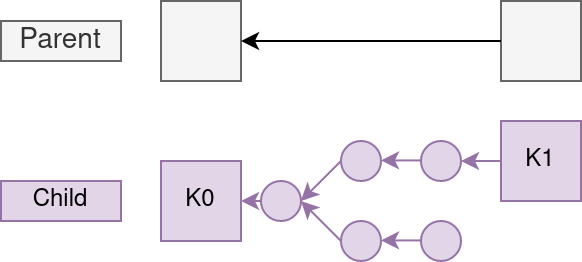
\includegraphics[scale=0.35]{microfork}
\end{figure}

\subsubsection{Generational forks}

This kind of attack is not a problem in PoW based BitcoinNG as producing
key blocks is a hard task. On the contrary key blocks on hyperchains are
extremely cheap — a malicious leader may flood the network with coinciding
key blocks:

\begin{figure}[h]
	\caption{Generational Fork}
	\centering
	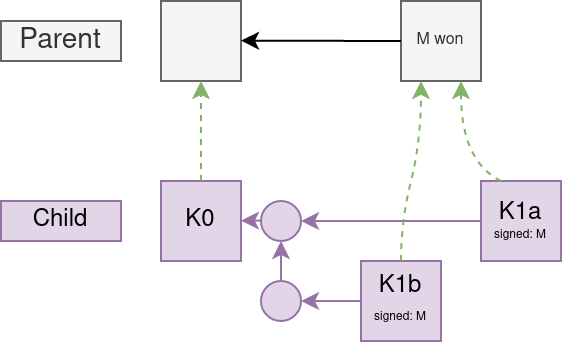
\includegraphics[scale=0.35]{genfork}
\end{figure}

The $K1a$, $K1b$, etc. are key blocks on the child chain emitted by a malicious
leader over different micro blocks. This
effectively splits the network into many parts, as it becomes unclear to which of
the forks the delegates should commit. To resolve this issue, a single leader
must be agreed upon using some additional mechanism — a new election
should be performed with the exclusion of the compromised delegate.

To notify the network about the generational fork, the peers need to announce
this fact on the parent chain by publishing fraud commitments and
cryptographic proofs of generational fraud (PoGF). Each commitment has to point to
the latest child key block considered valid by delegates or,
 in other words, to the generation where the fork starts. The committer also needs
to declare to which fork they want to contribute — if they get elected, they
will be required to build on it (we disallow rollbacks). The voting power should be
calculated based on the latest block before the fraud was detected.


\begin{figure}[h]
	\caption{Generational Fork Solving}
	\centering
	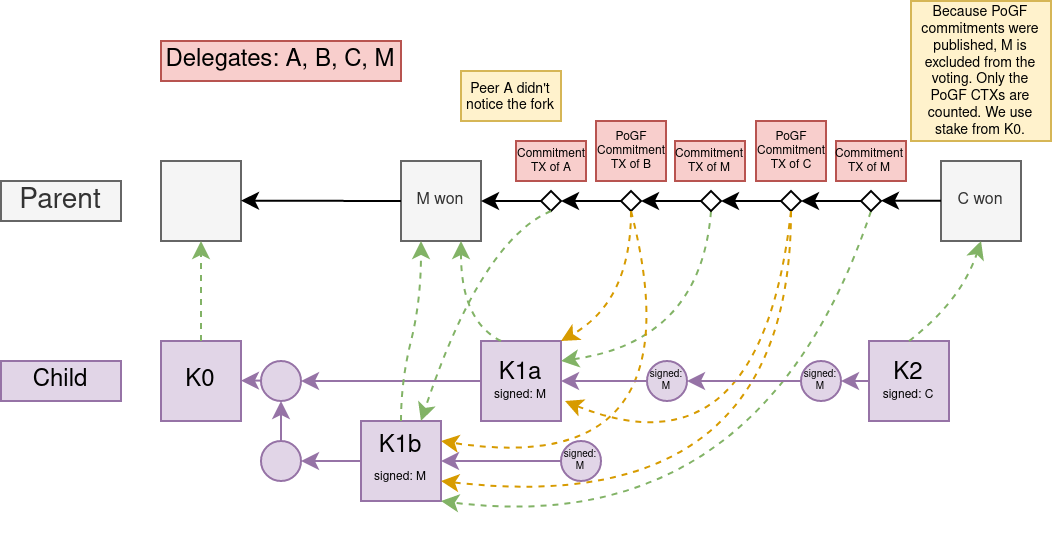
\includegraphics[scale=0.45]{genfraud}
\end{figure}

Due to network propagation
delays and connectivity failures, some nodes might not notice that a generational
fork was created and not respond accordingly. New nodes or the ones catching up
after downtime, need recognize that a generational fork was created and apply
the appropriate solution. Some of them may commit to one of the forks and receive a fraud
notification after they start mining. Therefore, we introduce a metric over the
branches that we call "difficulty" for a conventional reason. The
rule to resolve conflicts caused by such data races is similar to the already
existing PoW strategy "follow the most difficult chain," and the formula is
as follows:

\begin{minipage}{\linewidth}
\begin{lstlisting}
  difficulty : Block -> Int
  difficulty(Genesis) = 0
  difficulty(block) =
    if(exists proof of generational fraud on /block/)
         sum of the voting power of delegates
           that committed to /prev(block)/ +
         sum of the voting power of delegates
           that committed to solve the genfork
    else sum of the voting power of delegates
           that committed to /prev(block)/
\end{lstlisting}
\end{minipage}

If two forks have the same difficulty, then the one with lower block hash
is selected. This formula ensures that key blocks pointing to a PoGF are always
strongly preferred over ordinary key blocks — delegates who detect generational
forks have higher priority over poorly connected/bootstrapping/syncing ones.

This solution is vulnerable to situations where the leader does not respond
or responds with significant delay. In these cases, a new election is held,
stalling the network for a while. To resolve the doubts arising when the
previous leader reappears,
finalization after $f$ (implementation–dependent) generations is introduced.

In particular case a malicious leader may submit a generational
fork by publishing key blocks on conflicting micro blocks.
In response we prioritize PoGF, because the consequences of forks on
key blocks are much more severe than those on micro blocks, and they would need to
be resolved anyway.

\subsection{Stake grinding}

Since the RNG depends ultimately on the key block hash on a PoW chain, it is
impossible to predict its outcomes. One could try to mine the parent chain
in a special way, but it would require so much computational power that in
most cases it would be easier to take control by a 51\% attack.

\subsection{Long–range attack}
While it is still possible to perform a long–range attack, it would be impossible to do it
secretly and without preparation since the very beginning. The commitments
guarantee that the information of delegates is stored on an immutable chain,
and one would need to announce their will of mining suspicious blocks during
the entire period of the attack. This would quickly expose the intention of the attacker
and let the others prepare for a possible upcoming attack
(by blacklisting them, for example).

\subsection{Avoiding punishments}
Transaction fees may vary depending on circumstances on the network.
Consequently, the original penalty system of BitcoinNG is not sufficient in
those cases, where the risk of fraud detection is much lesser than expected profit.

One of the most natural ideas is to freeze the stake for some period before the
election. In this scenario, the protocol is able to painfully slash
malicious leaders by burning/redistributing their stake. However, this may raise
some problems when delegated voting is used — malicious leader may vote
for their second, empty account that will commit the fraud, losing potentially
nothing if compromised. This can be dealt with, allowing only
top $k$ stakers to be voted on or slashing \textit{everyone} who supported the
malicious leader. We leave this issue implementation–dependent as different solutions
require different security approaches.
